\section{Ideas of GAN}
生成对抗网络由一个生成网络(Generator)与一个判别网络(discriminator)组成. 生成网络从潜在空间(latent space)中随机取样作为输入, 其输出结果需要尽量模仿训练集中的真实样本. 判别网络的输入则为真实样本或生成网络的输出, 其目的是将生成网络的输出从真实样本中尽可能分辨出来. 而生成网络则要尽可能地欺骗判别网络. 两个网络相互对抗, 不断调整参数, 最终目的是使判别网络无法判断生成网络的输出结果是否真实. 

在提出GAN的论文中, Goodfellow将Generator比作制造假钞的罪犯, 而Discriminator是验钞警察, 在Generator和Discriminator之间的相互对抗, 相互成长, 直至验钞警察分辨不出假钞团伙制造的假钞为止, Generator的训练便是成功了. 也有一种比较和平的比喻, 将Generator比作学生, 将Discriminator比作老师. 相互成长, 共同进步.
\begin{quotation}
    The generative model can be thought of as analogous to a team of counterfeiters, trying to produce fake currency and use it without detection, while the discriminative model is analogous to the police, trying to detect the counterfeit currency. Competition in this game drives both teams to improve their methods until the counterfeits are indistiguishable from the genuine articles.
\end{quotation}

\begin{figure}[!htbp]
    \centering
    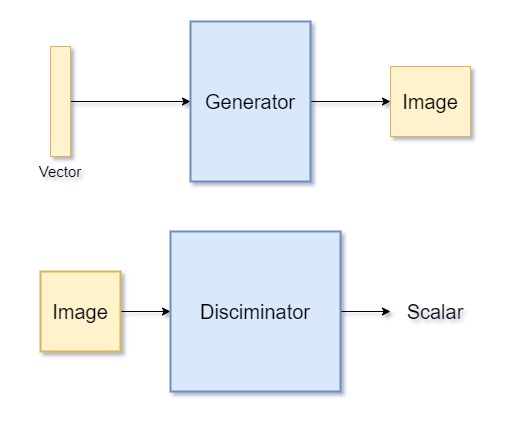
\includegraphics[height=15em]{pic/pic0201.jpg}
    \caption{G and D}
    \label{fig:0201}
\end{figure}
GAN原理如图~\ref{fig:0201}所示, 以图像生成为例, 将vector输入至Generator生成fakeImage, 再将从Dataset中的抽样出的数据image和fakeIamge输入至Discriminator, 输出一个0-1的标量. 当fakeImage越接近image时, scalar越接近1; 同理, 当fakeImage越假, Scalar越接近0.

\subsection{Algorithm of GAN}
第一步, 先固定G, 通过随机生成网络参数, 一开始G生成的假图像质量比较低, 和真实图像差别较大. 之后使用假图片和从数据集中随机抽取的真实图像来训练D, 使D可以给真实图像高分, 给生成的假图像低分. 如图~\ref{fig:0202}所示:
\begin{figure}[!htbp]
    \centering
    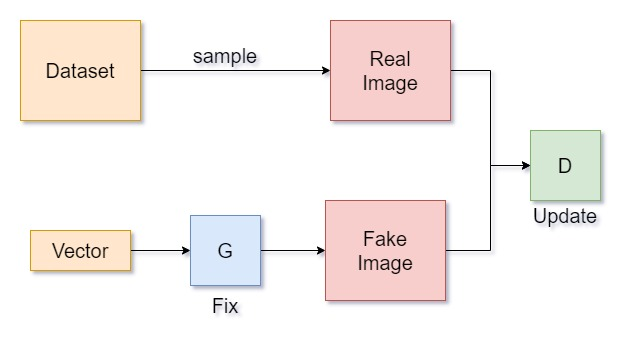
\includegraphics[height=10em]{pic/pic0202.jpg}
    \caption{Step01 Fix G Update D}
    \label{fig:0202}
\end{figure}

第二步, 固定上一步训练好的D, 更新G的参数, 让G生成的图片被D打高分, 如图~\ref{fig:0203}所示:
\begin{figure}[!htbp]
    \centering
    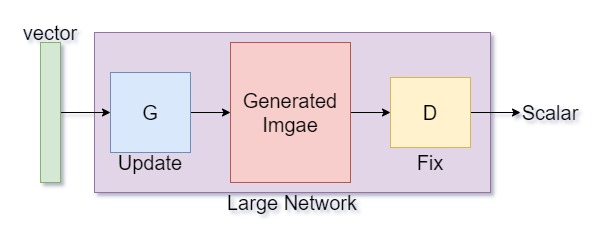
\includegraphics[height=10em]{pic/pic0203.jpg}
    \caption{Step02 Fix D Update G}
    \label{fig:0203}
\end{figure}

将上述两步总结, 则在每一个训练的迭代中:
\begin{itemize}
    \item 从数据库取 $m$ 个样本(Real Image) ${x^{1}, x^{2}, ..., x^{m}}$
    \item 取样 $m$ 个输入向量 ${z^{1}, z^{2}, ..., z^{m}}$
    \item 得到生成数据 ${\tilde{x}^{1}, \tilde{x}^{2}, ..., \tilde{x}^{m}}$, $\tilde{x}^{i}=G(z^{i})$
    \item 更新D的参数$\theta_{D}$, 使$\tilde{V}$最大, $\tilde{V}=\frac{1}{m}\sum_{i=1}^{m}logD(x^{i})+\frac{1}{m}log(1-D(\tilde{x}^{i}))$
    \item $\theta_{D} \gets \theta_{D} + \eta\nabla\tilde{V}(\theta_{D})$
    \item 取样 $m$ 个输入向量 ${z^{1}, z^{2}, ..., z^{m}}$
    \item 更新G参数$\theta_{G}$使$\tilde{V}$最大, $\tilde{V}=\frac{1}{m}\sum_{i=1}^{m}logD(G(z^{i}))$
    \item $\theta_{G} \gets \theta_{G} + \eta\nabla\tilde{V}(\theta_{G})$
\end{itemize}

\subsection{Generator learn by itself?}
有Auto-encoder的先例(可用作PCA), 如图~\ref{fig:0204}所示, 可以将其中的Decoder部分当作Generator, 但这种Generator在没有Discirminator的情况下, 会出现一些意想不到的结果. 
\begin{figure}[!htbp]
    \centering
    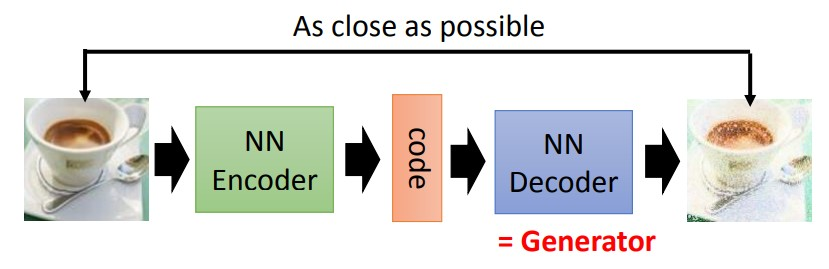
\includegraphics[height=10em]{pic/pic0204.jpg}
    \caption{Auto-Encoder}
    \label{fig:0204}
\end{figure}

另外对于生成网络Generator来讲, 往往最后一层为全连接层, 如图~\ref{fig:0205}所示: , 最后生成图像的每一个像素事比较独立, 没有较强关联性, 因此从根本上可能会出现一些噪声性质的纹理. 
\begin{figure}[!htbp]
    \centering
    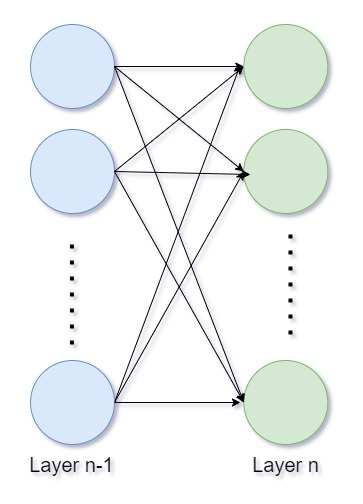
\includegraphics[height=15em]{pic/pic0205.jpg}
    \caption{G layer}
    \label{fig:0205}
\end{figure}

\subsection{Discriminator to generate?}
训练好判别器Discriminator需要质量高的假生成数据, 而只有把判别器Discriminator训练好, 模型才知道什么是质量高的假生成数据. 因此需要各种假设.

假设我们可以找到质量高的假生成数据, 则训练D为求解
$$ \tilde{X}=arg \max \limits_{x} D(x)$$
最终训练结果是让生成器G生成数据的分布尽可能接近真实数据. 但仅用Discriminator训练, 当网络有一定深度时, 很难求解上式. 因此使用生成器来生成假数据, 在深度学习之前, 普遍使用条件随机场等方法先假设分布, 之后再解.

总结两小节, 生成器Generator优点在于可以生成, 但是它没有大局观, 往往包含一定噪声, 而且很难去学习到相邻像素之间的关系; 而Discriminator优势在于评判, 对整体性把握比较好(可以使用CNN), 但对于高质量假图像的生成, 可行性不高. 

% \begin{figure}[!htbp]
%     \centering
%     \subfloat[BC]{\label{fig:0105a}
%     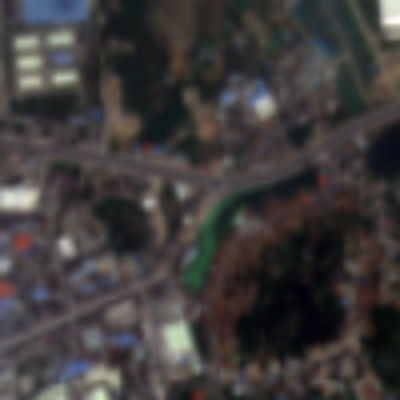
\includegraphics[height=10em]{pic/img5_LR_bicubic.jpg}}
%     \quad
%     \subfloat[SR]{\label{fig:0105b}
%     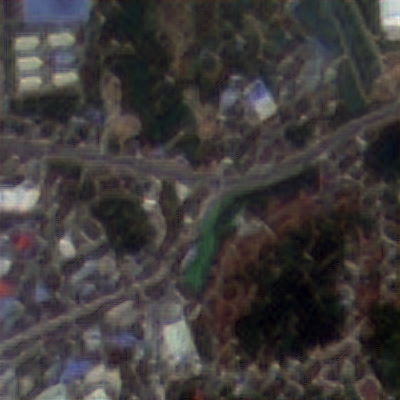
\includegraphics[height=10em]{pic/img5_SR.jpg}}
%     \quad
%     \subfloat[GT]{\label{fig:0105c}
%     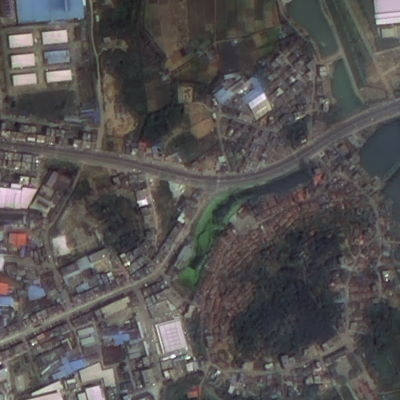
\includegraphics[height=10em]{pic/img5_GT.jpg}}
%     \caption{result05}
%     \label{fig:0105}
% \end{figure}